\subsection{Coxeter arrangements in $\Hbb^3$}

Since the second half of the 1st semester, I have been investigating Coxeter arrangements of rank 3 and 4 Coxeter groups of hyperbolic signature.
The nature of this investigation has been informed by the fact that a lot of progress in this field has been made by looking at relevant pictures.
Accordingly, I have developed a set of tools to visualise Coxeter arrangements in $\Hbb^2$ and $\Hbb^3$ using Mathematica.
Developing such tools also has the advantage of providing tangible examples on which to try ideas, and was a good way to learn hyperbolic geometry.
In the following, let $G_{353}$ and $G_{555}$ be Coxeter groups corresponding to the following $\Gamma$.
\[
	G_{353} \leftrightsquigarrow
	\begin{tikzpicture}
		\def\size{0.7}
		\tikzstyle{every label}=[font=\footnotesize]
		\tikzstyle{every node}=[font=\footnotesize]

		% First square nodes
		\node[FSC] (l)	at (0,0)	{};
		\node[FSC] (ml)	at ($(l)+(\size,0)$)	{};
		\node[FSC] (mr)	at ($(ml)+(\size,0)$)	{};
		\node[FSC] (r)	at ($(mr)+(\size,0)$)	{};

		\draw (l) to node[above] {3} (ml);
		\draw (ml) to node[above] {5} (mr);
		\draw (mr) to node[above] {3} (r);
	\end{tikzpicture}\;,
	\quad
	\quad
	G_{555} \leftrightsquigarrow
	\begin{tikzpicture}[baseline={(c.base)}]
		\def\size{0.7}
		\tikzstyle{every label}=[font=\footnotesize]
		\tikzstyle{every node}=[font=\footnotesize]

		% First square nodes
		\node[FSC] (c)	at (0,0)	{};
		\node[FSC] (t)	at ($(c)+(0,\size)$)	{};
		\node[FSC] (r)	at ($(c)+(0.83*\size,-0.83*\size)$)	{};
		\node[FSC] (l)	at ($(c)+(-0.83*\size,-0.83*\size)$)	{};

		\draw (c) to node[left] {5} (t);
		\draw (c) to node[right, near start] {5} (r);
		\draw (c) to node[left, near start] {5} (l);
	\end{tikzpicture}
\]

It turns out that $G_{353}$ is the only rank 4 Coxeter system for which the $K(\pi,1)$ conjecture is open.
It also happens to be geometrically well-behaved, in that its fundamental domain in $\Hbb^3$ is compact and of finite volume.

The geometry of a rank 4 hyperbolic Coxeter group is determined by 6 interplanar angles.
In Euclidean space, if these interplanar angles do correspond to some tetrahedron, then it is relatively simple to find a specific tetrahedron that realises these angles.
In $\Hbb^3$, this is more complicated, since angles are specific scale.
We developed a way to symbolically compute tetrahedrons in $\Hbb^3$ corresponding to any appropriate Coxeter group.

We used this to realise a specific model for $G_{353}$.
In \cref{fig:353_origin}, we show 120  cells (many of which are at the back of the plot and not visible) in the Coxeter arrangement for $G_{353}$ that have a vertex at the origin.
The chosen fundamental chamber has an edge along the $z$-axis in blue.
The faces of the fundamental chamber were coloured red, green, blue and orange, and we considered the Coxeter element that corresponded to the product of those faces in that order.
The edges of the fundamental chamber were also coloured in a unique way.
In \cref{fig:353_origin}, we only see orange faces since the cells shown are the orbit under the subgroup generated by the red, green and blue faces of the fundamental chamber, and we see 120 cells because that is the order of that parabolic subgroup.

\begin{figure}
	\centering
	\begin{subfigure}[t]{.45\textwidth}
		\centering
		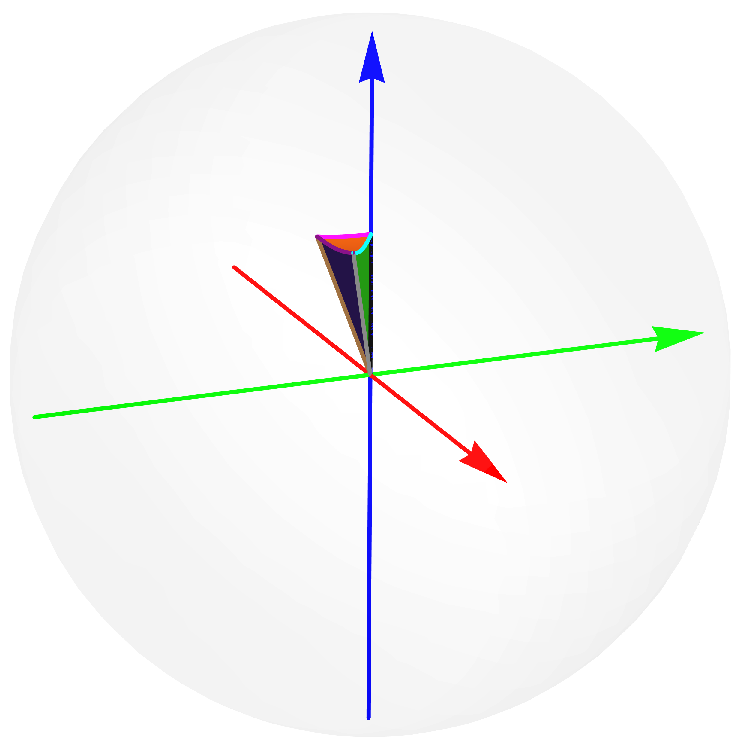
\includegraphics[width=6cm]{353_fundchamber.pdf}
		\caption{Our chosen fundamental chamber for $G_{353}$.}
		\label{fig:353_fund_chamber}
	\end{subfigure}
	\hspace{0.2ex}
	\begin{subfigure}[t]{.45\textwidth}
		\centering
		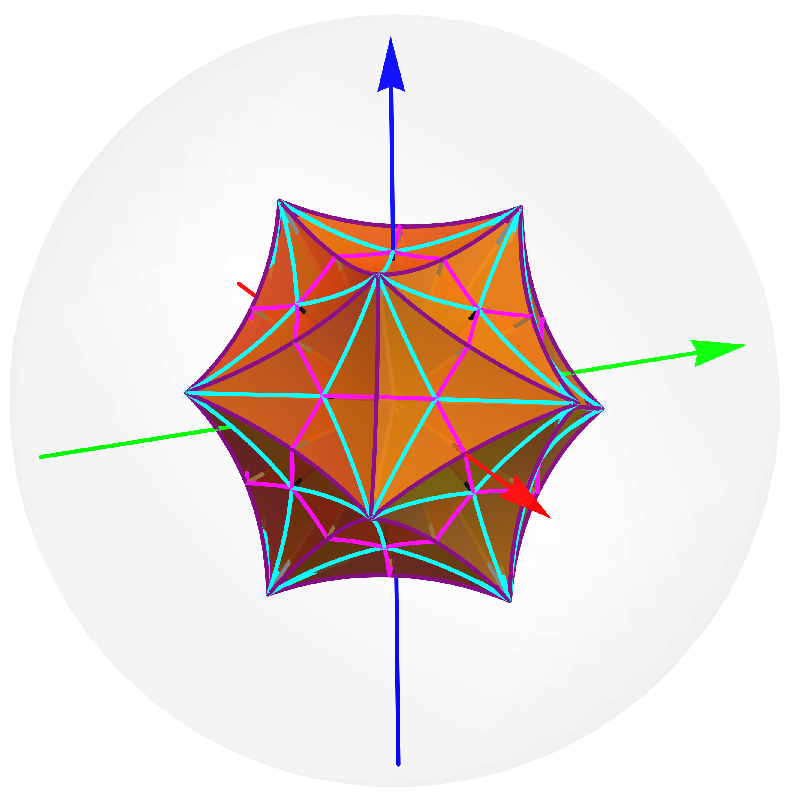
\includegraphics[width=6cm]{353_origin.pdf}
		\caption{A part of the Coxeter arrangement for $G_{353}$ consisting of 120 copies of the fundamental chamber that are positioned at the origin.}
		\label{fig:353_origin}
	\end{subfigure}%
	\caption{Realising the Coxeter arrangement for $G_{353}$.}
	\label{fig:test}
\end{figure}

In \cref{fig:353_cut}, we see a cut of the Coxeter arrangement of $G_{353}$ along a plane in  $\Hbb^3$.
For this, we initially plotted significantly more cells of the Coxeter arrangement than in  \cref{fig:353_origin}.
This is an irregular tiling of $\Hbb^2$.
In the case of  $G_{353}$, taking different cuts reveals the same tiling up to translation.

In \cref{fig:353_coxeter_axis}, we see the Coxeter axis corresponding to the product of the red, green, blue and orange planes of the fundamental chamber in that order.
Alongside this, we see some cells that lie along the Coxeter axis.
Such cells are important as any reflection factorisation of a Coxeter element that makes a tetrahedron must be one of these cells.

\begin{figure}
	\centering
	\begin{minipage}{.5\textwidth}
		\centering
		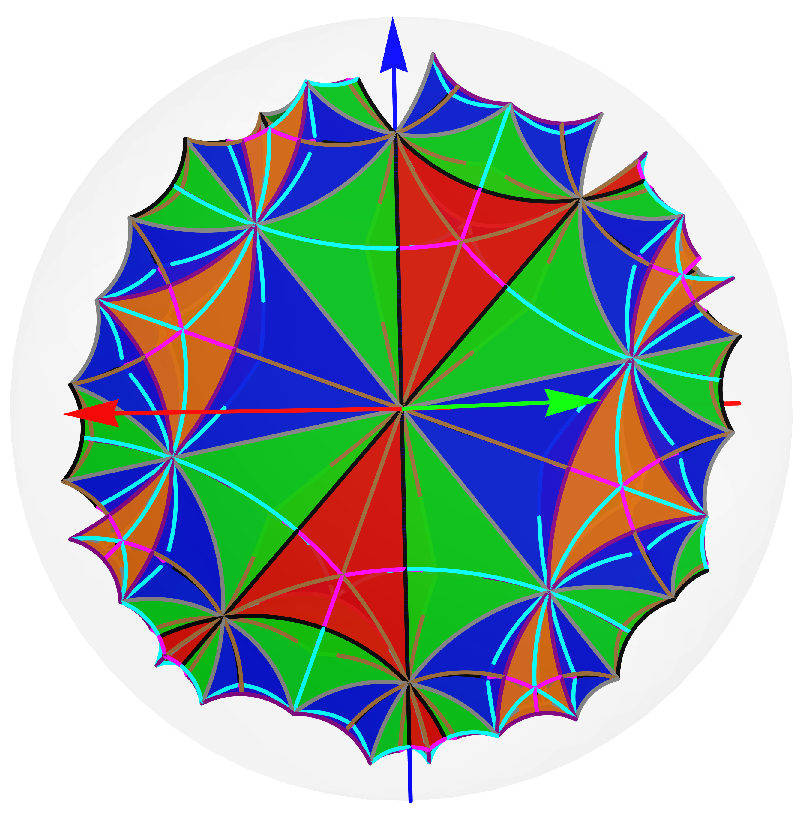
\includegraphics[width=6cm]{353_cut.pdf}
		\caption{A cut of the Coxeter arrangement of $G_{353}$ along a plane in $\Hbb^3$.}
		\label{fig:353_cut}
	\end{minipage}%
	\begin{minipage}{.5\textwidth}
		\centering
		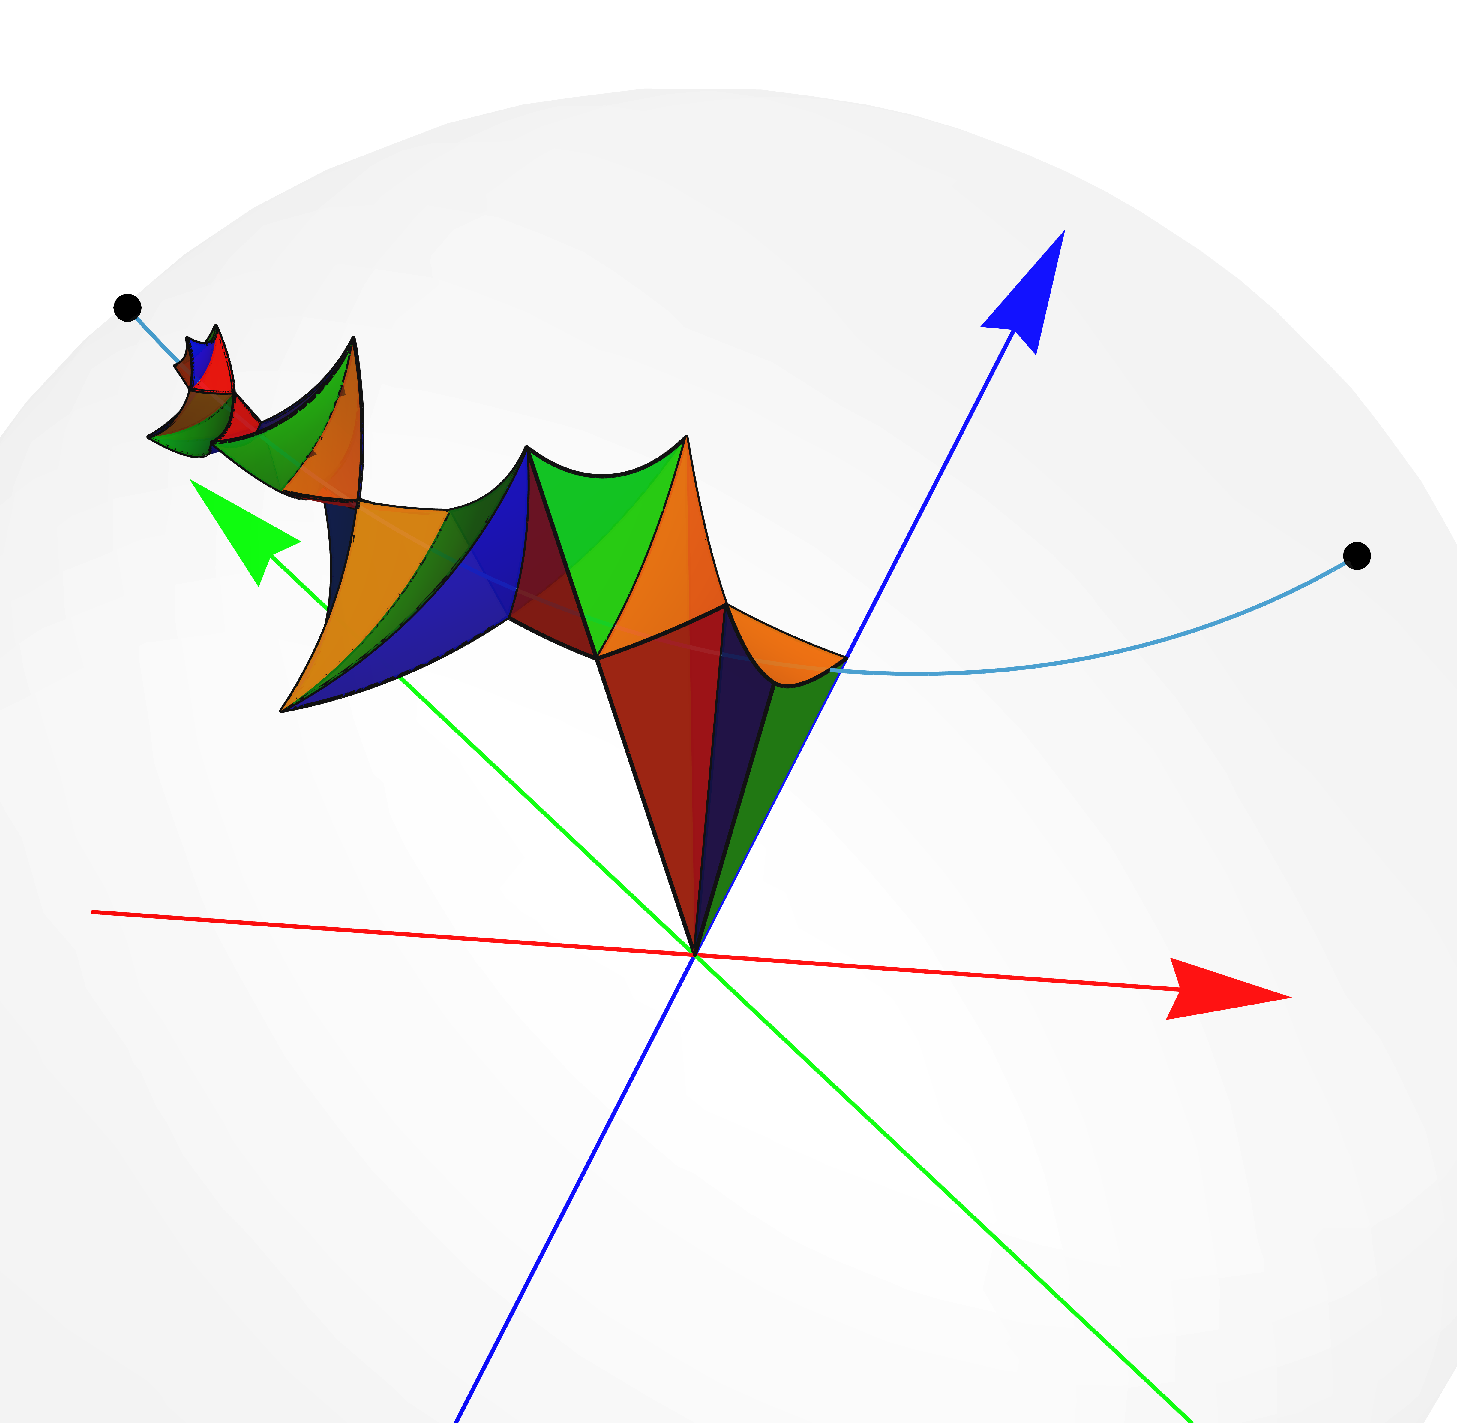
\includegraphics[width=6cm]{353_coxeteraxis.pdf}
		\caption{The Coxeter axis Corresponding to a Coxeter element in $G_{353}$, as well as some cells that lie along this Coxeter axis.}
		\label{fig:353_coxeter_axis}
	\end{minipage}
\end{figure}

We were not able to use these tools to prove anything about $G_{353}$, but in developing these plots and the geometric tools needed to make them, I gained a lot of intuition and knowledge for these hyperbolic arrangements.
We were also able to compute some closed forms for certain geometric constructions in $\Hbb^2$ and  $\Hbb^3$ useful for future calculations.
For example, we may denote planes in $\Hbb^3$ as $p = (\mathbf{n},r)$, where $\mathbf{n}$ and $r$ are a normal vector and non-negative real respectively, such that the circle of intersection of $p$ with the unit sphere is the same as the circle of intersection of the plane $\mathbf{n} \cdot \mathbf{x} = r$ with the unit sphere.
In this notation, the reflection of the plane $p_1 =(\mathbf{n_1},r)$ through $p_2 = (\mathbf{n_2},s)$ with $\mathbf{n_1}=(x,y,z)$ and  $\mathbf{n_2}=(a,b,c)$ is
\begin{align*}
	 & {\scriptscriptstyle R_{p_2}(p_1) =\bigg(\text{Sign}\left(r(1+s^2)-2s(\mathbf{n_1}\cdot\mathbf{n_2})\right)\; \text{Normalise}\big[}                      \\
	 & {\scriptscriptstyle\quad 2ars + (1-s^2)x-2(a^2x+aby+acz),                                                                                             }  \\
	 & {\scriptscriptstyle\quad 2brs + (1-s^2)y-2(b^2y+abx+bcz),                                                                                             }  \\
	 & {\scriptscriptstyle\quad 2crs + (1-s^2)z-2(c^2z+acx+bcy) \;\big],                                                                                      } \\
	 & {\scriptscriptstyle\sqrt{\frac{r^2 (1 + s^2)^2 - 4 r s (1 + s^2) (\mathbf{n_1}\cdot\mathbf{n_2}) +
					4 s^2 ((-1 + c^2) (-1 + y^2) + 2 a c x z + (-1 + 2 c^2) z^2 +
					2 b y (a x + c z) + b^2 (-1 + 2 y^2 + z^2))}{1 + s^4 -
					4 r s (\mathbf{n_1}\cdot\mathbf{n_2}) - 4 r s^3 (\mathbf{n_1}\cdot\mathbf{n_2}) +
					s^2 (2 + 4 r^2 - 4 y^2 + 8 a c x z - 4 z^2 + 8 b y (a x + c z) +
					4 b^2 (-1 + 2 y^2 + z^2) + 4 c^2 (-1 + y^2 + 2 z^2))}}\,\bigg)}.
\end{align*}

We also investigated

